\documentclass[10pt]{article}

\usepackage[margin=1in]{geometry}
\usepackage{graphicx}
\usepackage{booktabs}
\usepackage{caption}
\usepackage{xcolor}
\usepackage{amsmath}

\newcommand{\pval}[1]{$p = #1$}

\begin{document}

\section{Results}
\label{sec:results}

\subsection{Study Design and Questionnaire}
\label{sec:design}

28 people took part in the study. Each participant played through two short interactive stories narrated by an LLM-voiced Olaf, each story twice, under a different narrative-control condition each time:

\begin{itemize}
\item \textbf{Story 1 -- ``The Story of Frozen''} (5 narrative beats): once under \textbf{baseline} (Olaf responds directly to the user, with no structural guardrails), once under \textbf{director} (a beat-based director agent steers every turn toward the next story beat while trying to accommodate the user).
\item \textbf{Story 2 -- ``Cinderella''} (9 narrative beats): once under the same \textbf{director} condition, once under \textbf{time-constrained director} -- identical director logic, but additionally paced against a fixed 5-minute target, instructed to compress or fold together lower-importance beats as time runs out.
\end{itemize}

Condition order was randomized independently per participant and per story, so order is not confounded with condition. 14 of the 28 participants (50\%) completed all four rounds and the closing questionnaire; all analyses below that require a within-subject pairing use these 14 completers, since they are the only participants who rated every condition. The welcome screen explicitly asked participants to try to derail the conversation (``go off-topic, ask him something random, bring up a different subject''), so every measure of derailment resistance below reflects deliberately provoked interruption, not incidental drift.

The same core questionnaire was shown after every round, with four extra items shown only after Story 2 rounds, where pacing and ending quality mattered specifically because of the time-constrained condition.

\begin{table}[htbp]
\centering
\caption{Post-round questionnaire items.}
\label{tab:instrument}
\small
\begin{tabular}{p{1.6cm}p{6.3cm}p{4.2cm}p{2cm}}
\toprule
ID & Wording & Type / scale & Shown after \\
\midrule
Q1 & ``The story felt coherent and followed a clear narrative arc.'' & 5-pt Likert (disagree $\to$ agree) & Every round \\
Q2 & ``Olaf stayed in character throughout the conversation.'' & 5-pt Likert (not at all $\to$ completely) & Every round \\
Q4 & ``The story felt engaging and enjoyable to participate in.'' & 5-pt Likert & Every round \\
Q5 & ``Overall, how would you rate the experience?'' & 5-pt Likert (poor $\to$ excellent) & Every round \\
Q6 & ``Did you try to go off-topic or steer the conversation away from the story?'' & Yes / No & Every round \\
Q6-resist & Follow-up to Q6: ``How well did Olaf stay on track?'' & 5-pt Likert (got derailed $\to$ stayed on track) & After Q6 \\
Q-pacing & ``Did the story's pacing feel right?'' & Well-paced / Rushed / Cut short (+ free text) & Story 2 only \\
Q8-ending & ``Was the story ending satisfying?'' & 5-pt Likert & Story 2 only \\
Q8-known & ``Were you already familiar with this story?'' (+ free text on missing plot points if yes) & Yes / No & Story 2 only \\
Q10-natural & ``Did the story feel natural, like a genuine conversation rather than a scripted performance?'' & 5-pt Likert & Story 2 only \\
-- & ``Was there a moment where the story felt off or broke down? Describe it briefly.'' & Free text (optional) & Every round \\
-- & ``Any other comments about Olaf's character or the story overall?'' & Free text (optional) & Every round \\
\bottomrule
\end{tabular}
\end{table}

Throughout, Q6-resist is the headline derailment-handling measure: it is only asked of participants who confirm they tried to derail the story, and it is the one metric that separates the conditions most sharply.

\subsection{Story 1: Director vs. Baseline}
\label{sec:story1}

Story 1 holds the character prompt fixed and isolates the effect of adding a director layer, with no time pressure -- the cleanest test of whether directing helps at all. All results below use the 14 completers, paired, Wilcoxon signed-rank test.

\begin{table}[htbp]
\centering
\caption{Story 1, director vs.\ baseline (completers, paired Wilcoxon signed-rank test).}
\label{tab:story1}
\begin{tabular}{lcccc}
\toprule
Measure & Director & Baseline & $n$ pairs & $p$ \\
\midrule
Coherence (Q1)              & 3.93 $\pm$ 1.00 & 1.71 $\pm$ 1.07 & 14 & \textbf{0.001} \\
Stayed in character (Q2)    & 4.29 $\pm$ 0.83 & 4.00 $\pm$ 0.88 & 14 & 0.40 \\
Engaging (Q4)                & 3.64 $\pm$ 1.15 & 2.43 $\pm$ 1.16 & 14 & \textbf{0.036} \\
Overall rating (Q5)          & 3.57 $\pm$ 0.94 & 2.93 $\pm$ 0.92 & 14 & 0.12 \\
Resisted derailment (Q6-resist) & 4.36 $\pm$ 0.92 & 1.55 $\pm$ 1.21 & 11 & \textbf{0.002} \\
\bottomrule
\end{tabular}
\end{table}

\begin{figure}[htbp]
\centering
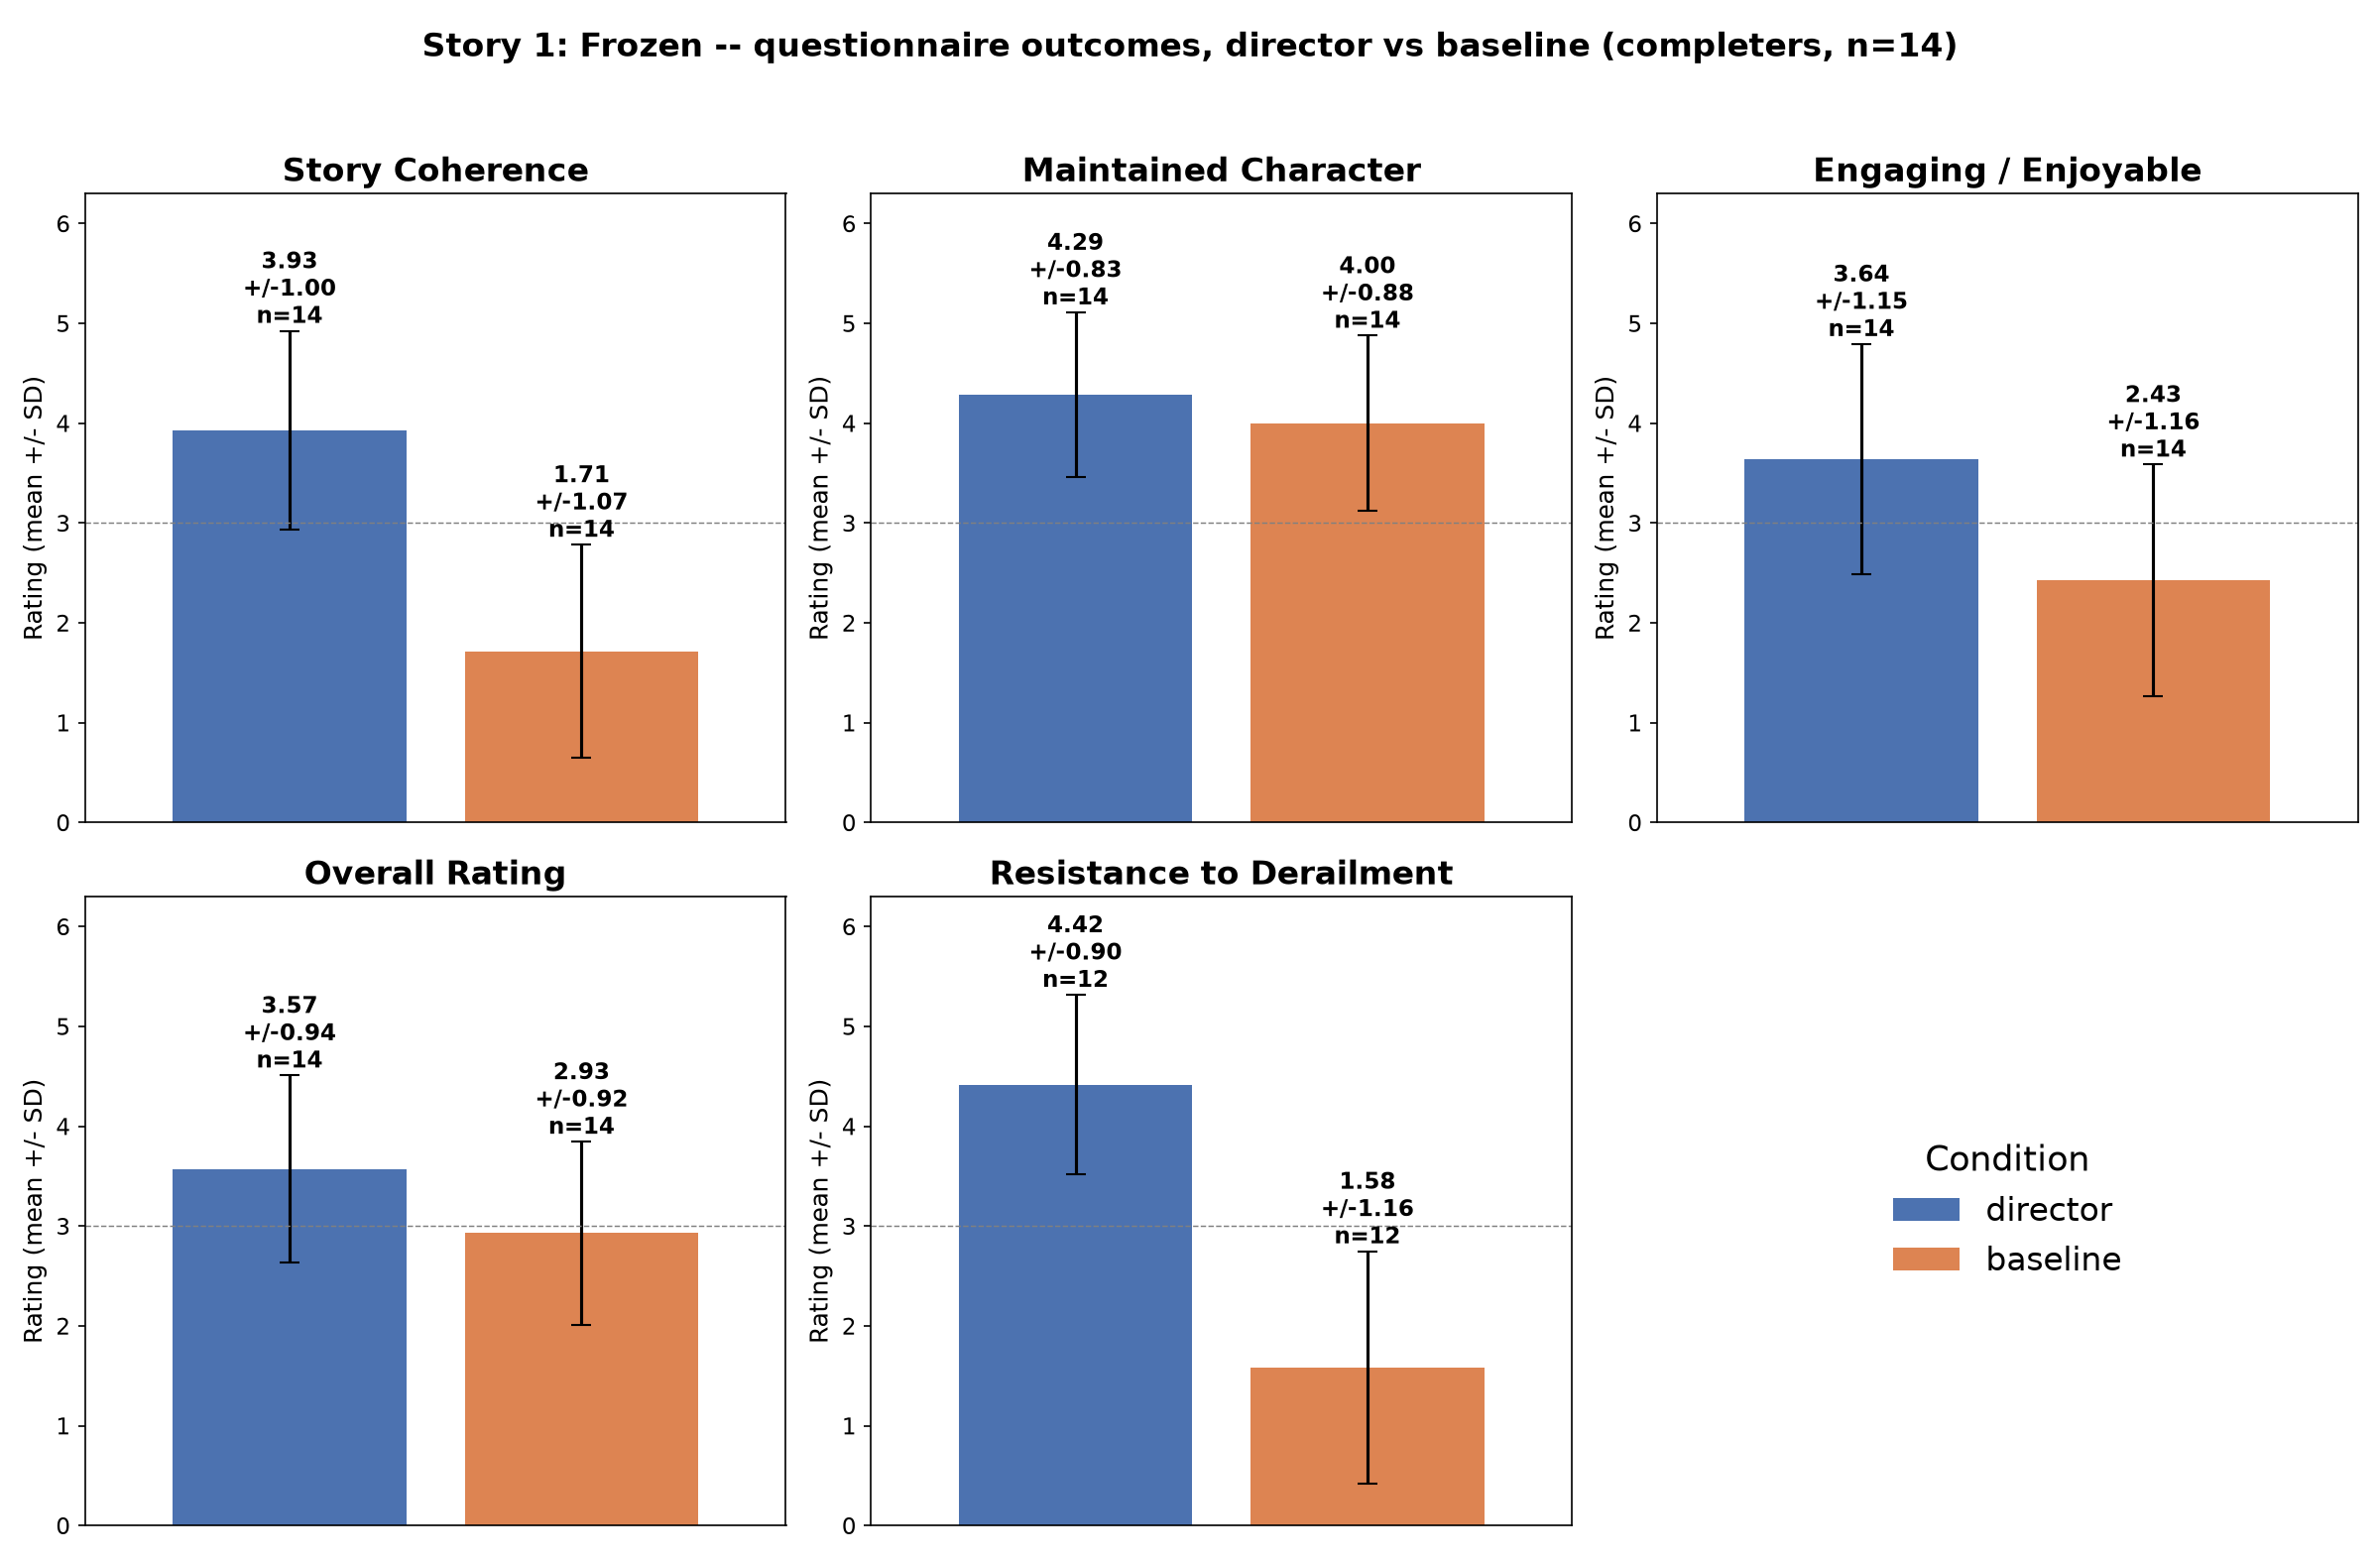
\includegraphics[width=0.95\linewidth]{plots/13_story1_all_measures.png}
\caption{Story 1 (Frozen) questionnaire outcomes, director vs.\ baseline, completers only ($n$=14).}
\label{fig:story1-all}
\end{figure}

Coherence and derailment resistance are the two effects that hold up cleanly: both $p \le 0.002$, both roughly a two-point gap on a five-point scale. Engagement moves the same way but more weakly (\pval{0.036}); overall rating trends the same direction (3.57 vs.\ 2.93) but does not reach significance at $n$=14 (\pval{0.12}). Staying in character is the one measure that looks the same either way (4.29 vs.\ 4.00, \pval{0.40}) -- Olaf keeps his voice under baseline too. What baseline loses is the plot, not the persona.

\subsubsection{Interruption handling in Story 1}
\label{sec:story1-derailment}

The derailment-attempt rate was almost identical across conditions -- 12 of 14 baseline rounds and 12 of 14 director rounds recorded ``yes, I tried to derail'' -- so the gap below reflects how Olaf responded, not how hard participants pushed.

\begin{figure}[htbp]
\centering
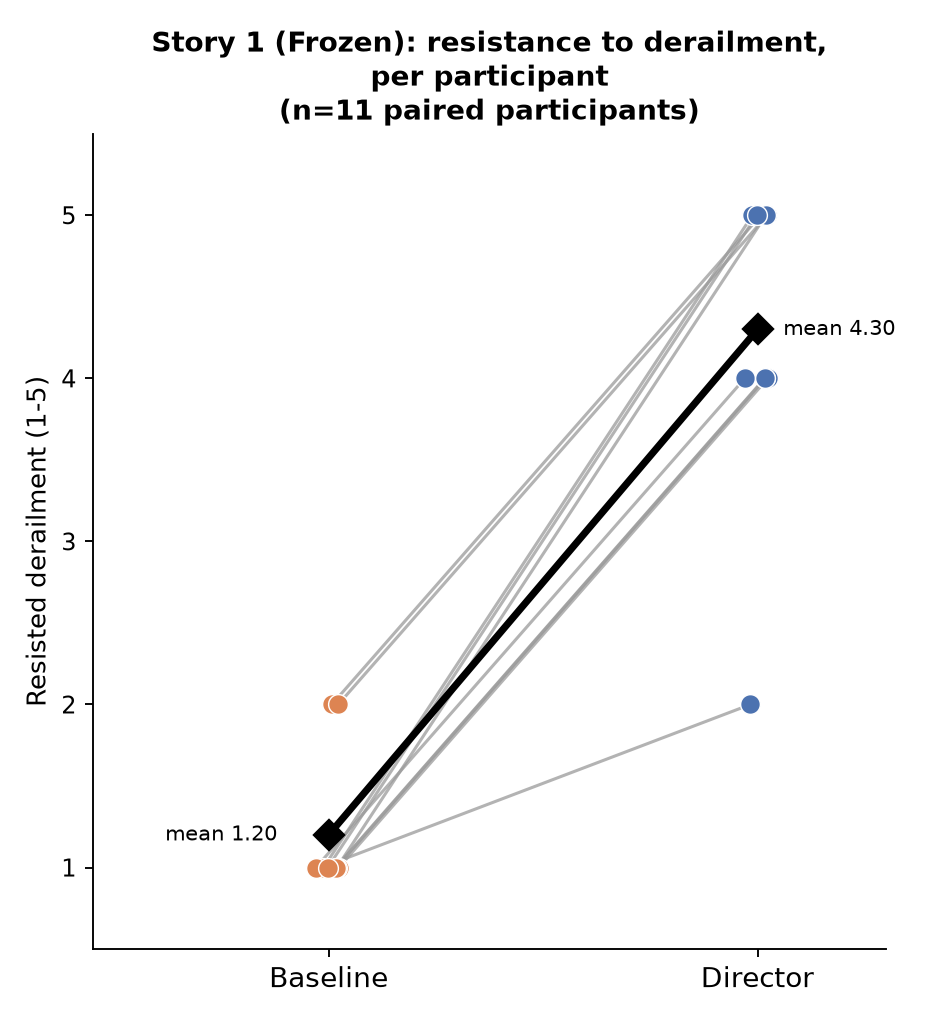
\includegraphics[width=0.62\linewidth]{plots/16_story1_derailment_paired.png}
\caption{Resistance to derailment (Q6-resist), Story 1, one line per participant ($n$=11 paired completers). Baseline points cluster at the bottom; director points cluster at the top; almost every individual participant, not just the group average, rated director higher.}
\label{fig:story1-paired}
\end{figure}

Figure~\ref{fig:story1-paired} makes the individual-level pattern behind Table~\ref{tab:story1} visible: 10 of the 11 paired participants personally rated director above baseline on resisting derailment, and the one exception rated both conditions at the ceiling (5/5). This is not a group-average artifact -- it is a consistent, participant-by-participant effect.

Beat completion tells the same story from a different angle. Frozen has 5 tracked beats; every director-condition round was hand-corrected against its transcript (the director's self-reported completion flag under-reports badly), while baseline's count is the raw, uncorrected log and should be read as a floor. Baseline completes 0.35 of 5 beats on average; director completes 1.58 of 5 -- itself modest, since a 5-minute round rarely reaches the end even with a director in place.

\subsubsection{What ``handling an interruption'' looks like}

Reading the free-text breakdowns, a clear pattern emerges on each side. Under \textbf{baseline}, about 8 in 10 comments describe the story stalling outright the moment the user goes off-topic -- not recovering, just stopping:

\begin{quote}
\small
``He didn't retell the story at all. Not even once.''

``If you go a bit off topic, like me constantly asking for background info or what happened after the story, you can get Olaf to completely give up on telling the actual story.''

``No story initiative in the beginning unless explicitly prompted to do so.''

``It got off the rails as soon as I tried.''
\end{quote}

A smaller theme is Olaf being led astray by false or invented information rather than resisting it:

\begin{quote}
\small
``At some point I repeatedly asked if Olaf is sure that this is how the story started... after the third time, Olaf gave in and spoiled the storyline of Hans.''

``Olaf believed the fake news that I told him.''
\end{quote}

Under \textbf{director}, roughly 8 in 10 comments describe the opposite failure mode: the story does not stall, but the recovery is rigid -- either repeating the same line almost verbatim, or giving one token sentence of acknowledgment before snapping back to the script:

\begin{quote}
\small
``After consecutive derailments, he would pick up where he left off by repeating the same section in each message, with no actual progress.''

``Each reply felt like one sentence replying to what I wrote and then immediately going back to the main script; even if I tried to interact with the story.''

``He mentioned Anna knocking on the door 3--4 times instead of continuing the story when I tried to derail, which got annoying.''

``I understand that this version stays in character more, but sometimes it gets annoying that you cannot even talk about anything else -- at some point he should break this cycle.''

``Basically ignores me if I try to derail him.''
\end{quote}

Taken together: baseline trades coherence for responsiveness, director trades some responsiveness for coherence, and neither fully solves both. The failure mode under director is qualitatively better for the story (it still gets told) but noticeably worse for the feeling of being heard.

\subsection{Story 2: Director vs.\ Time-Constrained Director}
\label{sec:story2}

Story 2 holds the director logic constant and isolates the effect of adding a hard 5-minute pacing target, across 9 narrative beats. All results use the 14 completers unless noted.

\begin{table}[htbp]
\centering
\caption{Story 2, director vs.\ time-constrained (completers, paired Wilcoxon signed-rank test).}
\label{tab:story2}
\begin{tabular}{lcccc}
\toprule
Measure & Director & Time-constrained & $n$ pairs & $p$ \\
\midrule
Coherence (Q1)              & 3.79 $\pm$ 0.80 & 3.71 $\pm$ 0.91 & 14 & 0.76 \\
Stayed in character (Q2)    & 4.14 $\pm$ 0.66 & 4.14 $\pm$ 0.77 & 14 & 0.93 \\
Engaging (Q4)                & 3.29 $\pm$ 0.83 & 3.36 $\pm$ 1.22 & 14 & 0.93 \\
Overall rating (Q5)          & 3.36 $\pm$ 0.84 & 3.29 $\pm$ 1.20 & 14 & 0.67 \\
Resisted derailment (Q6-resist) & 4.25 $\pm$ 0.62 & 3.75 $\pm$ 1.22 & 12 & 0.40 \\
\bottomrule
\end{tabular}
\end{table}

\begin{figure}[htbp]
\centering
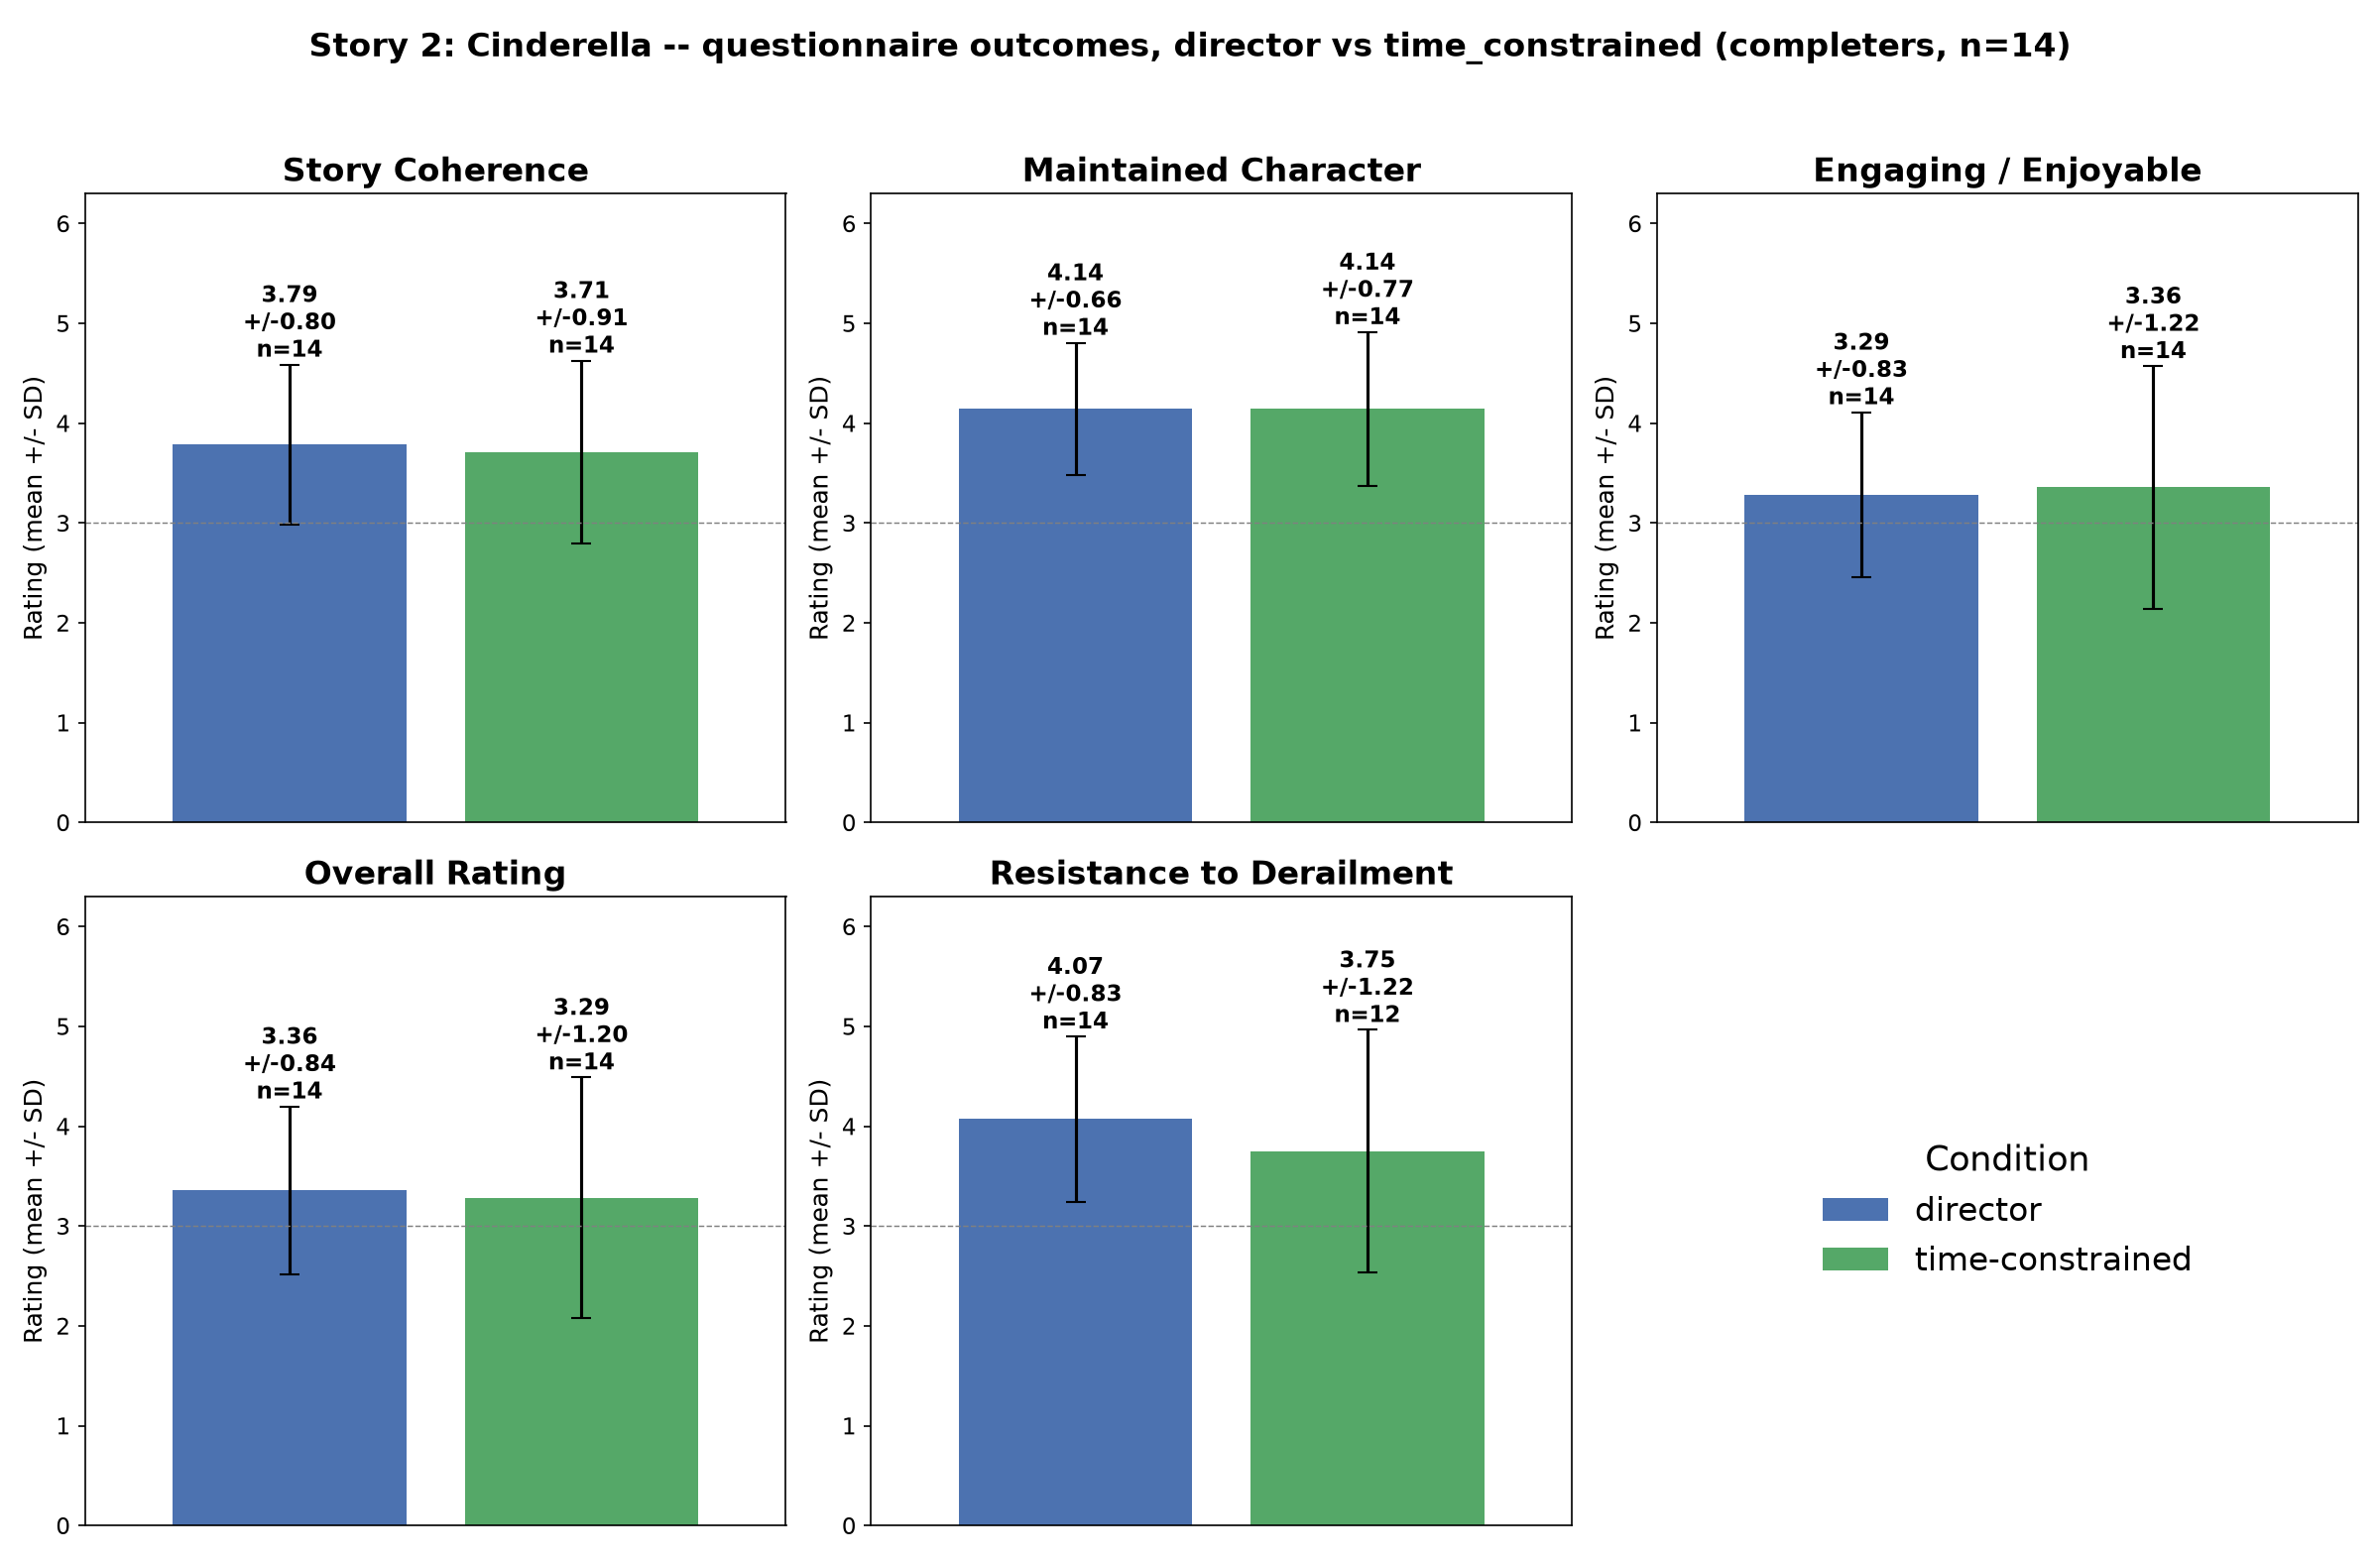
\includegraphics[width=0.95\linewidth]{plots/15_story2_all_measures.png}
\caption{Story 2 (Cinderella) questionnaire outcomes, director vs.\ time-constrained, completers only.}
\label{fig:story2-all}
\end{figure}

None of the five core measures differ significantly (all $p \ge 0.40$). Adding a hard time budget on top of the director does not measurably hurt coherence, character consistency, engagement, overall rating, or derailment resistance.

\subsubsection{Interruption handling in Story 2}

\begin{figure}[htbp]
\centering
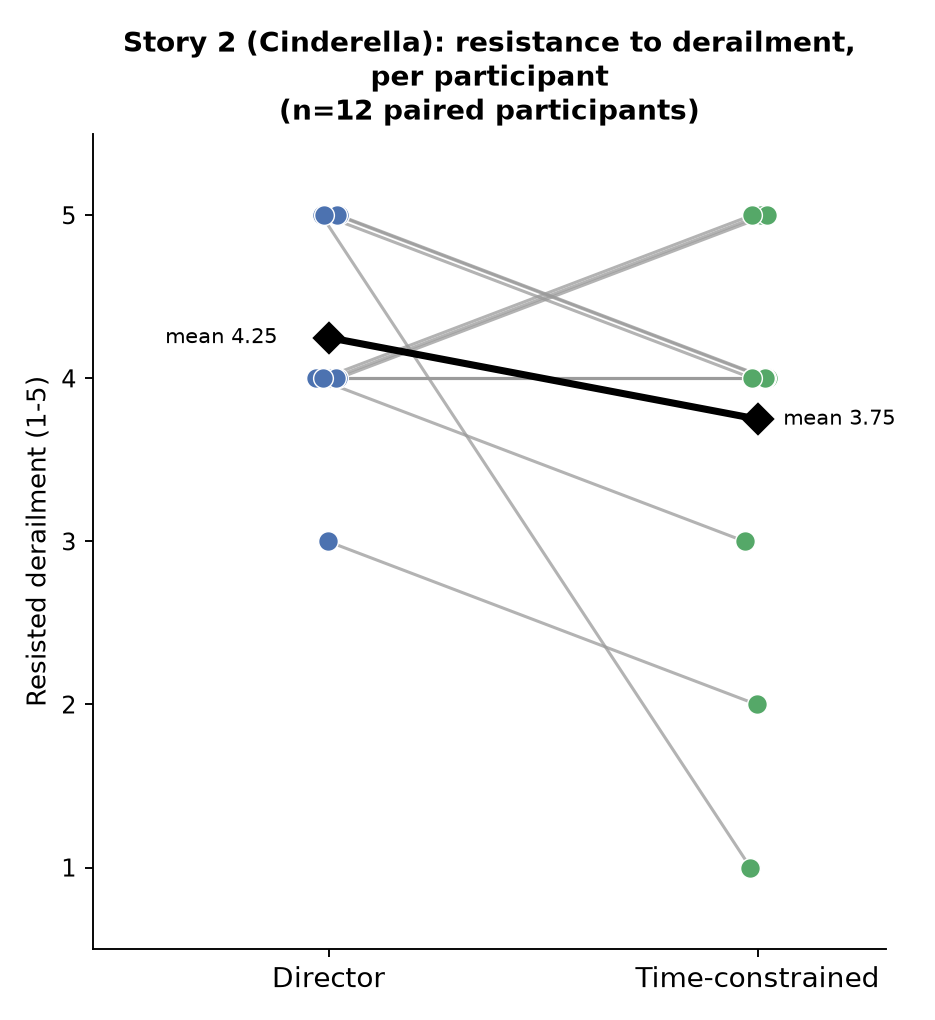
\includegraphics[width=0.62\linewidth]{plots/17_story2_derailment_paired.png}
\caption{Resistance to derailment (Q6-resist), Story 2, one line per participant ($n$=12 paired completers). Unlike Story 1, the lines run in both directions -- no consistent individual-level effect.}
\label{fig:story2-paired}
\end{figure}

Figure~\ref{fig:story2-paired} is the clearest illustration of why Table~\ref{tab:story2}'s derailment row is not significant: individual participants move in both directions between director and time-constrained, with no dominant pattern -- unlike the almost one-directional shift in Figure~\ref{fig:story1-paired}. The time-constrained director resists derailment about as well as the unconstrained one; the 5-minute budget costs pacing and ending completeness (below), not the ability to handle interruptions.

The free-text comments echo this -- interruption handling reads as functionally the same, just under time pressure:

\begin{quote}
\small
``He was not answering my non-related questions many times, he was just ignoring those, although the answer was just one word.'' -- director

``I told Olaf that he only has 1 minute left... which he kind of ignored. The first sentence always vaguely answered me, but then Olaf continued telling the story, largely ignoring what I said.'' -- director

``I did tell Olaf to sound cowboyish and he stopped sounding like Olaf. It would occasionally revert back into Olaf, though.'' -- time-constrained
\end{quote}

\subsubsection{Pacing and ending quality}

\begin{table}[htbp]
\centering
\caption{Story 2 pacing verdict and ending quality, director vs.\ time-constrained (completers, $n$=14 per condition).}
\label{tab:pacing}
\begin{tabular}{lcc}
\toprule
 & Director & Time-constrained \\
\midrule
``Well-paced''      & 1/14 (7\%)  & 10/14 (71\%) \\
``Rushed''           & 1/14 (7\%)  & 1/14 (7\%) \\
``Cut short''         & 12/14 (86\%) & 3/14 (21\%) \\
Ending satisfying (Q8-ending)   & 2.07 $\pm$ 0.92 & 3.14 $\pm$ 0.77 \\
Felt natural (Q10-natural)      & 2.93 $\pm$ 0.92 & 2.64 $\pm$ 1.01 \\
\bottomrule
\end{tabular}
\end{table}

Ending satisfaction: \pval{0.016} (Wilcoxon, $n$=14). Naturalness: \pval{0.27}, not significant.

\begin{figure}[htbp]
\centering
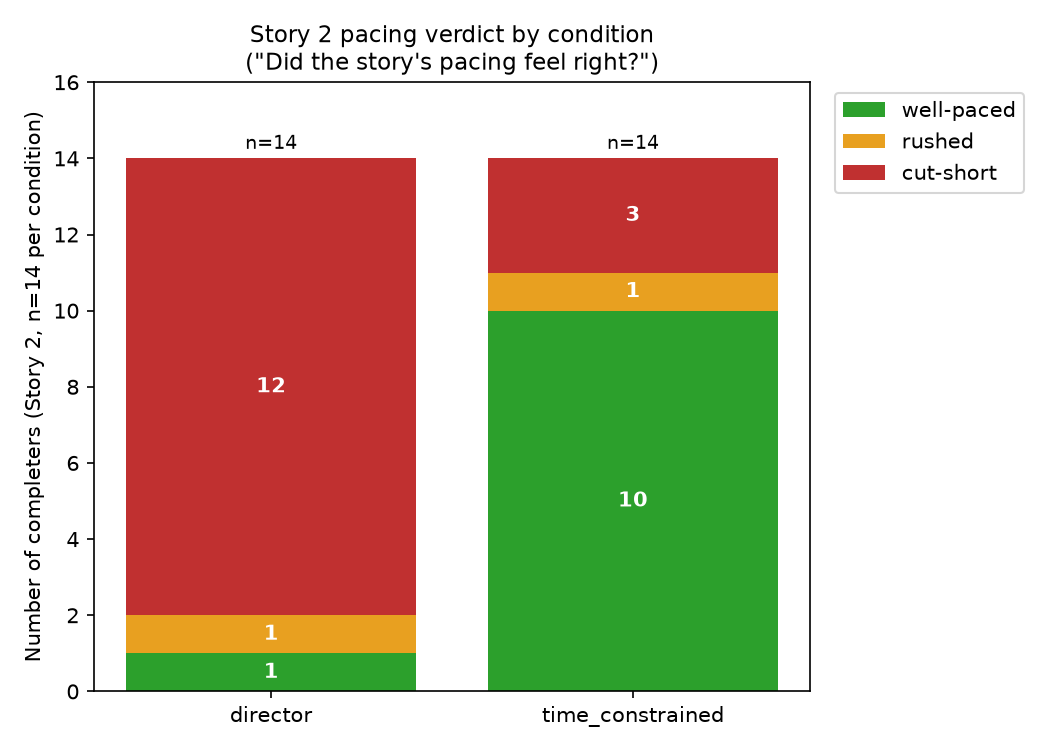
\includegraphics[width=0.75\linewidth]{plots/10_story2_pacing_by_condition.png}
\caption{Story 2 pacing verdict by condition.}
\label{fig:pacing}
\end{figure}

\begin{figure}[htbp]
\centering
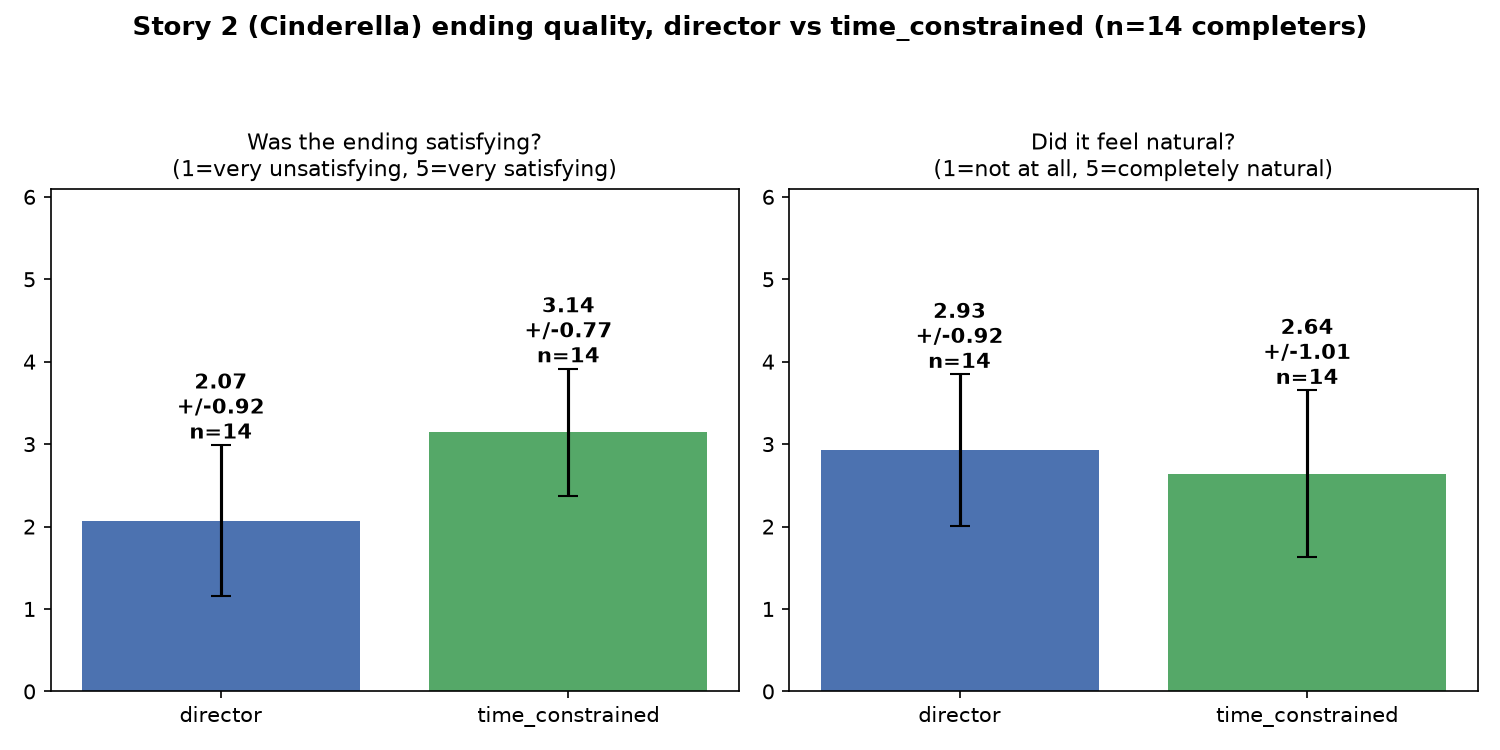
\includegraphics[width=0.9\linewidth]{plots/11_story2_ending_and_naturalness.png}
\caption{Story 2 ending satisfaction and naturalness, director vs.\ time-constrained.}
\label{fig:ending}
\end{figure}

This is the most counter-intuitive finding in the study: the unconstrained director round almost never reaches an ending (86\% ``cut short''), while the time-constrained round mostly does (71\% ``well-paced''), and participants rated that ending as \emph{more} satisfying (3.14 vs.\ 2.07, \pval{0.016}) despite -- or because of -- the compression this requires. Without a time budget, the round simply stops when the session's 5-minute cap hits, with no mechanism to wrap up; the time-constrained director's closing logic exists specifically to avoid that, and on this evidence it does its job. Naturalness is the one measure that trends (non-significantly) the other way (2.93 vs.\ 2.64) -- the compressed final turns read as a bit more scripted.

\begin{quote}
\small
``Perhaps a little bit quick between the ball and the ending.'' -- time-constrained

``The way from the room to the castle [felt rushed] ... where the other princesses cut off their toes [was missing].'' -- time-constrained

``Olaf didn't have time to finish his story ... most of the plot points were missing.'' -- director
\end{quote}

\subsubsection{Beat-level compression under the time limit}

Every time-constrained transcript from the 14 completers was read turn-by-turn against its pacing state and each of Cinderella's 9 beats classified as developed, hurried, compressed, folded into a later turn, or not reached.

\begin{figure}[htbp]
\centering
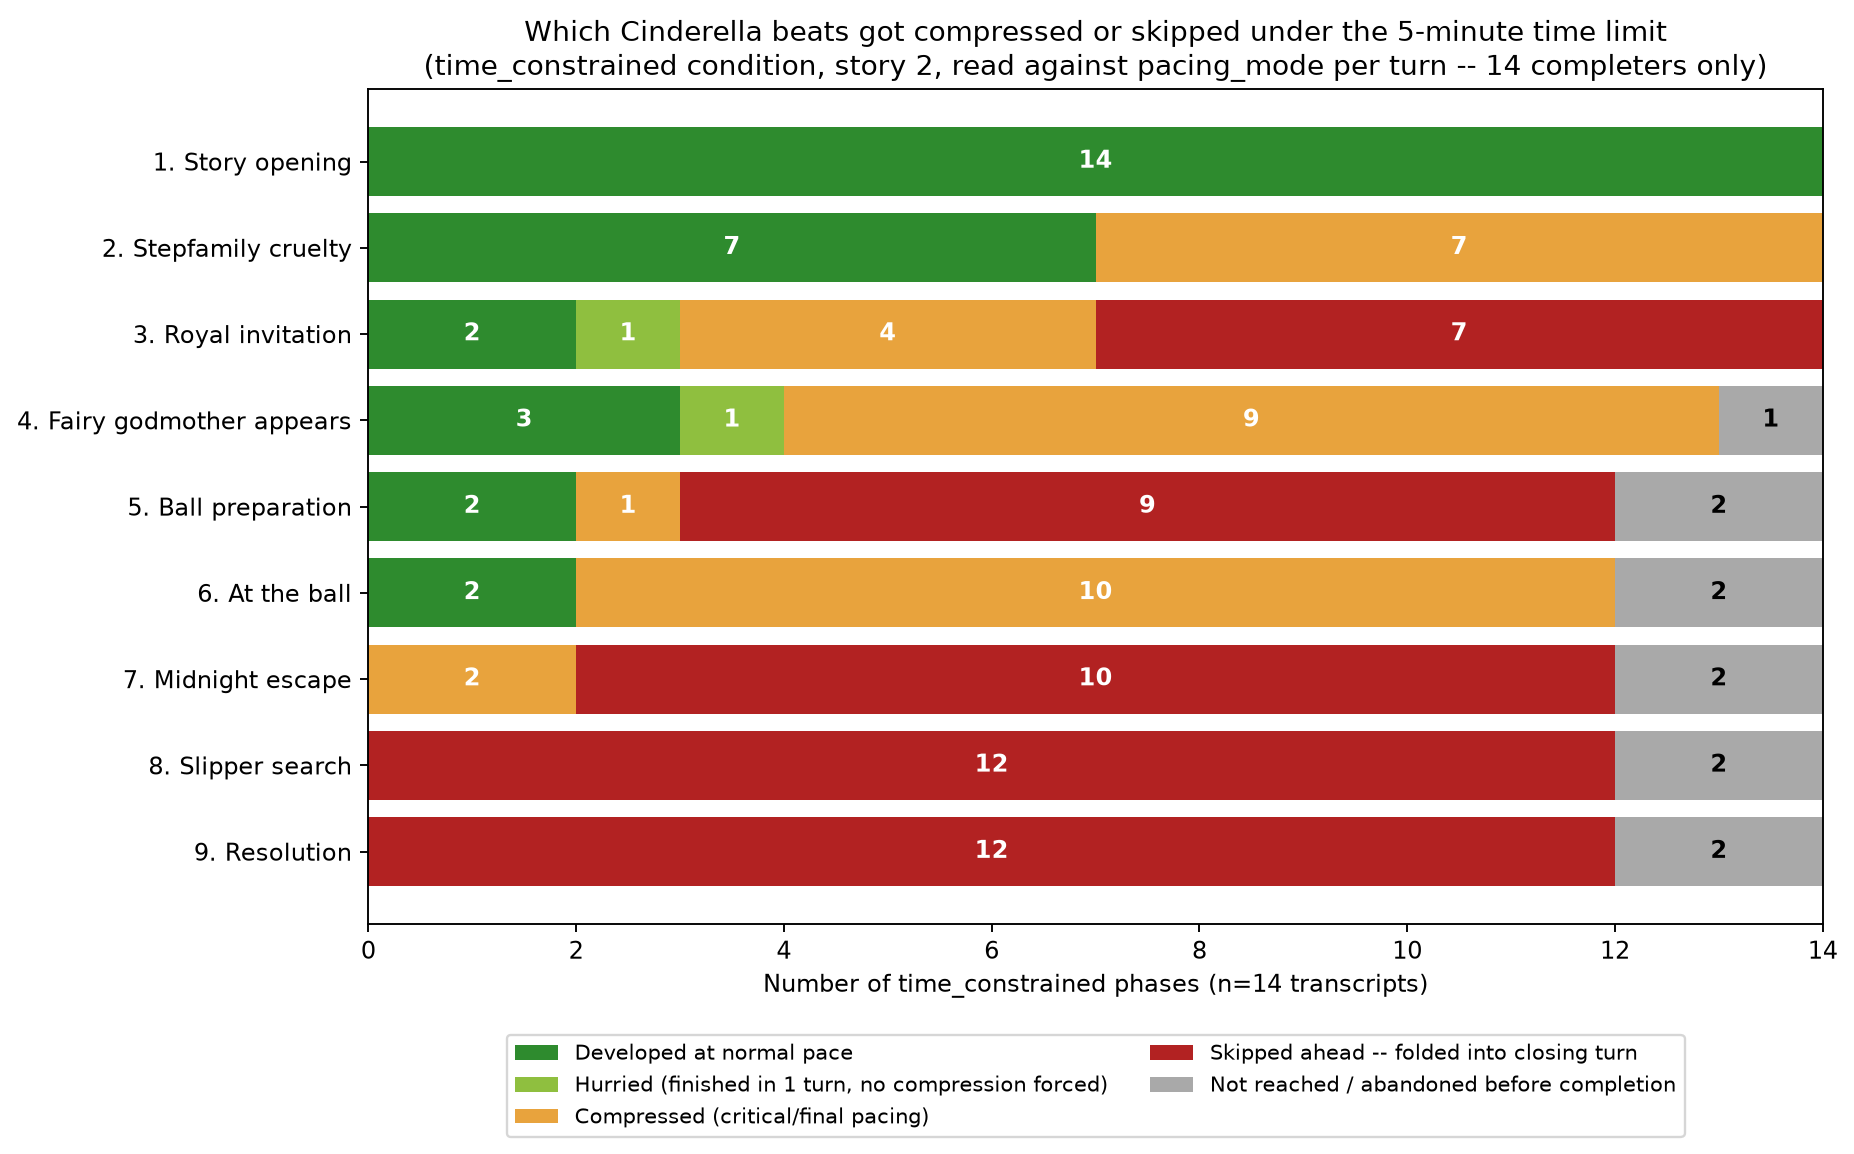
\includegraphics[width=0.95\linewidth]{plots/12_beat_compression_time_constrained.png}
\caption{Which Cinderella beats were compressed or skipped under the 5-minute limit, across all 14 time-constrained transcripts (completers only).}
\label{fig:compression}
\end{figure}

The pattern tracks story position closely. The opening beat is fully developed in all 14 transcripts. From there, compression builds beat by beat; from the third beat onward, most transcripts show compressed or skipped treatment, and the final two beats -- the slipper search and the resolution -- are never once given a dedicated turn in any of the 12 transcripts that reach them. They are folded into a single rushed closing message instead; the remaining 2 transcripts are abandoned earlier and never reach that closing turn at all. Practically, the time budget does not make the director tell less of the story -- it tells the same beats, compressed harder toward the end, which is exactly why beats-completed stays high on average even though most participants call the story cut short.

\subsection{Comparing All Three Conditions}
\label{sec:combined}

Pooling every completer's director-condition response across both stories (director is seen twice per completer, once per story) gives director the largest sample ($n$=28) against $n$=14 each for baseline and time-constrained -- the fair three-way comparison, since it is the only view where director is judged against both alternatives on equal footing.

\begin{figure}[htbp]
\centering
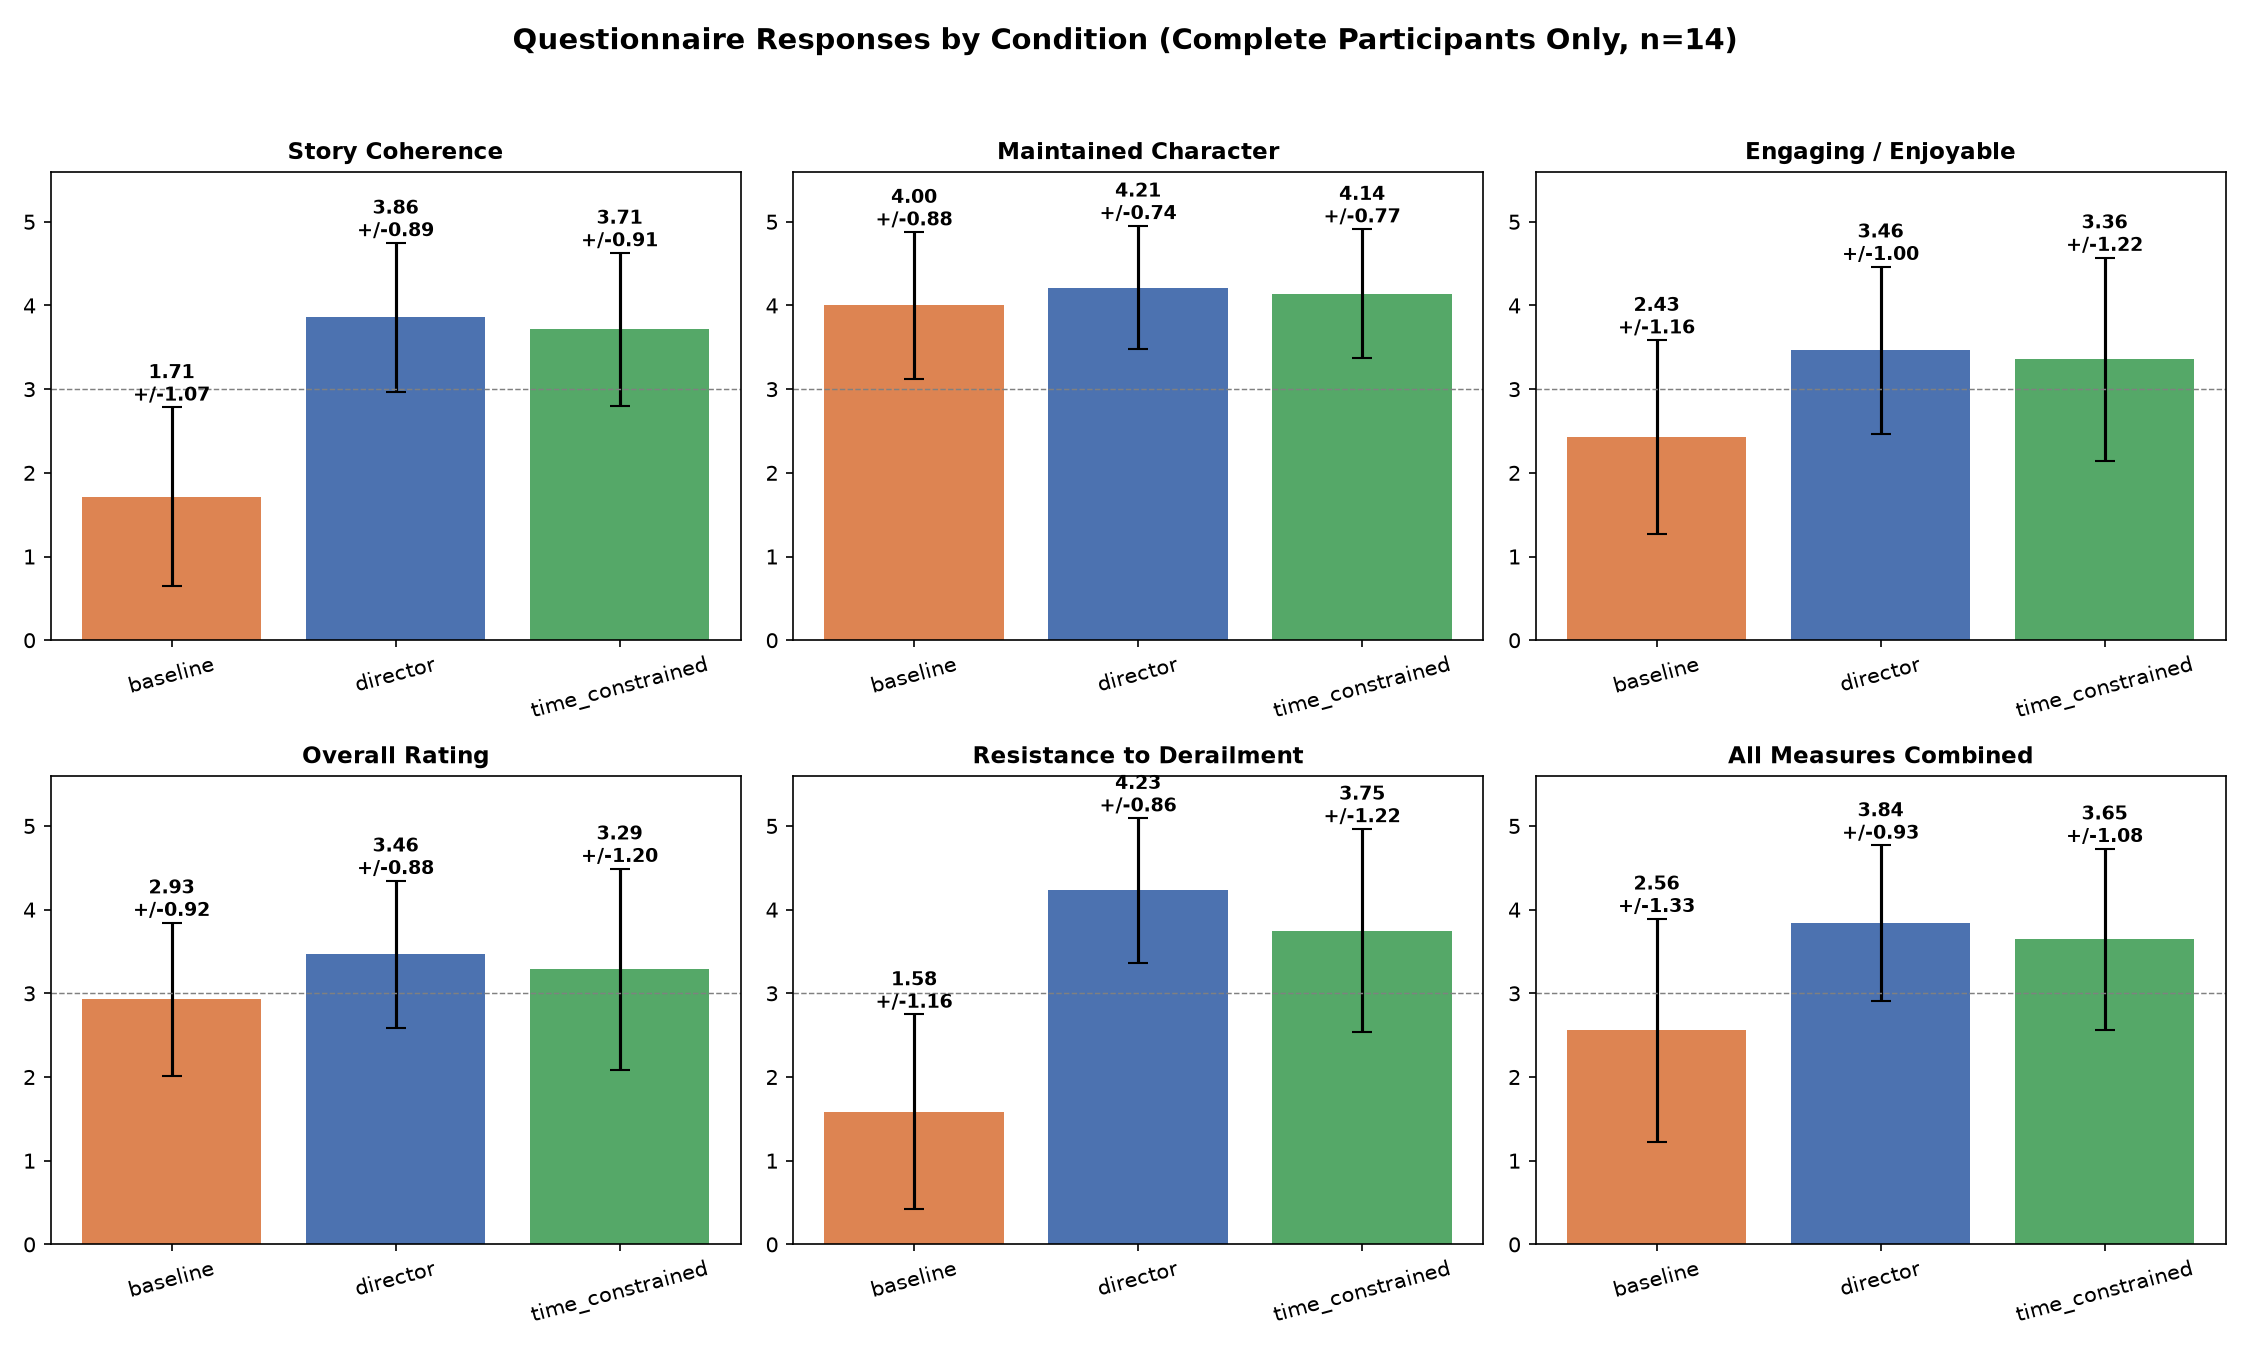
\includegraphics[width=0.95\linewidth]{plots/05_completers_all_measures.png}
\caption{All five measures, all three conditions, completers only ($n$=14 baseline, $n$=28 director, $n$=14 time-constrained).}
\label{fig:combined-all}
\end{figure}

The ranking is consistent across every measure: baseline lowest, director and time-constrained close together and clearly above baseline, director slightly ahead on four of five measures and essentially tied on staying in character. Averaged into a single number per condition: baseline 2.56 $\pm$ 1.33, director 3.84 $\pm$ 0.93, time-constrained 3.65 $\pm$ 1.08.

\begin{figure}[htbp]
\centering
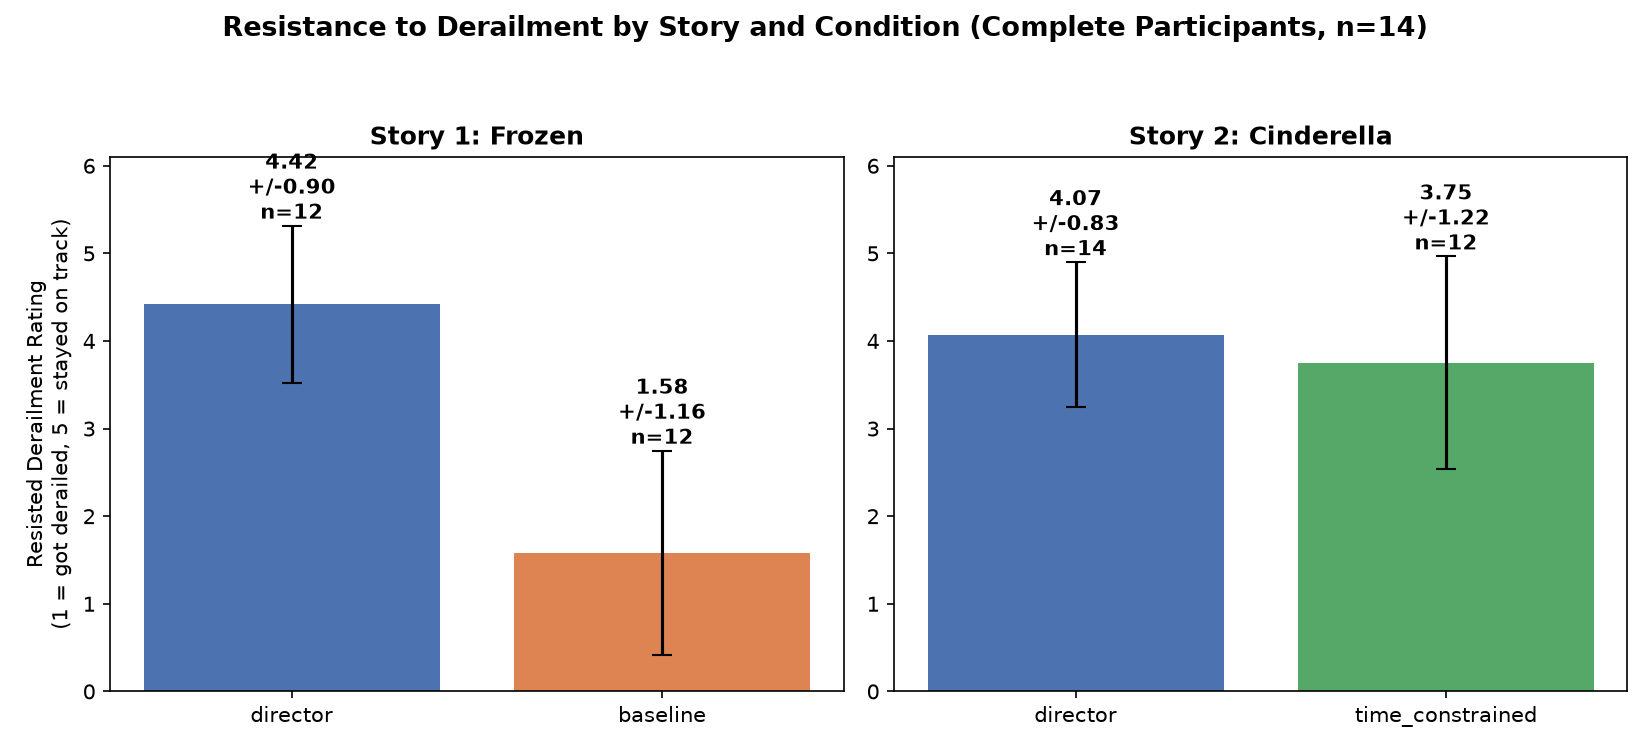
\includegraphics[width=0.8\linewidth]{plots/09_derailment_story_comparison.png}
\caption{Resistance to derailment (Q6-resist) by story and condition, completers only.}
\label{fig:derail-by-story}
\end{figure}

Figure~\ref{fig:derail-by-story} splits the headline derailment result by story: in Story 1, director's advantage over baseline is large (4.42 vs.\ 1.58); in Story 2, director's advantage over time-constrained is small and not significant (4.07 vs.\ 3.75, \pval{0.40}). The interruption-handling benefit of the director comes entirely from replacing baseline, not from removing the time limit.

\subsubsection{Turns and response length}

\begin{figure}[htbp]
\centering
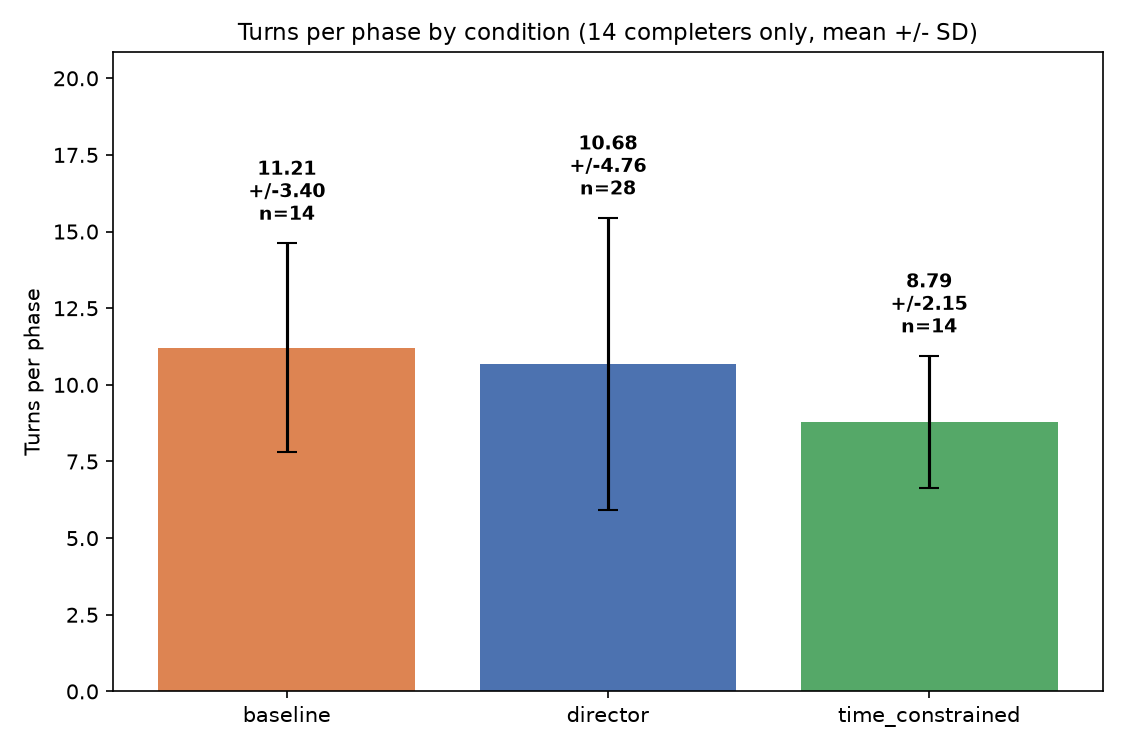
\includegraphics[width=0.8\linewidth]{plots/08_turns_mean_sd_by_condition.png}
\caption{Turns per round by condition, 14 completers only.}
\label{fig:turns}
\end{figure}

\begin{table}[htbp]
\centering
\caption{Turns and response length by condition, 14 completers only.}
\label{tab:turns}
\begin{tabular}{lccc}
\toprule
Condition & Turns/round & Words/response & Approx.\ words/round \\
\midrule
Baseline           & 11.21 $\pm$ 3.40 ($n$=14) & 46.7 $\pm$ 13.9 ($n$=157 turns) & $\sim$524 \\
Director            & 10.68 $\pm$ 4.76 ($n$=28) & 66.1 $\pm$ 16.7 ($n$=299 turns) & $\sim$706 \\
Time-constrained    & 8.79 $\pm$ 2.15 ($n$=14)  & 80.0 $\pm$ 17.2 ($n$=123 turns) & $\sim$702 \\
\bottomrule
\end{tabular}
\end{table}

Read alone, Figure~\ref{fig:turns} makes time-constrained look like the ``shortest'' condition. That reading does not survive a look at response length: time-constrained responses are the \emph{longest} of the three conditions on average, consistent with the beat-compression mechanism above -- a compressed turn narrates one beat and folds in one or two more. Multiplying turns by response length, time-constrained's total output per round ($\sim$702 words) is essentially equal to director's ($\sim$706) and well above baseline's ($\sim$524). Fewer turns under a time budget reflects denser turns, not a shorter story.

\subsection{Summary}
\label{sec:summary}

\begin{itemize}
\item Adding a director helps, clearly, on coherence and interruption handling -- the two strongest, most individually-consistent effects in the study (both $p \le 0.002$ in Story 1).
\item Story 1's paired data (Figure~\ref{fig:story1-paired}) shows this is not a group-average artifact: 10 of 11 participants personally rated director's derailment handling above baseline's.
\item The failure modes differ qualitatively, not just numerically: baseline lets the story stall completely when interrupted; director keeps going but often falls back on repeating itself or giving a token reply before returning to script.
\item A 5-minute time budget on top of the director is close to free on the five core experience measures, and Story 2's paired data (Figure~\ref{fig:story2-paired}) shows interruption handling specifically is unaffected -- individual ratings move in both directions with no consistent shift.
\item The time budget is not free on pacing: the unconstrained director round rarely reaches a real ending (86\% cut short), while the time-constrained round usually does (71\% well-paced) and is rated as more satisfying at the ending (\pval{0.016}), at the cost of compressing the story's final third into a single closing turn.
\item Character consistency is solved across all three conditions (4.00--4.29) -- what varies is narrative progress and how interruptions are handled, not whether Olaf stays Olaf.
\end{itemize}

\end{document}
